\documentclass{article}
\usepackage[utf8]{inputenc}
\usepackage[T1]{fontenc}
\usepackage{xcolor}
\usepackage{amsmath}
\usepackage{amssymb}
\usepackage{tikz}
\usetikzlibrary{calc,positioning}

\begin{document}

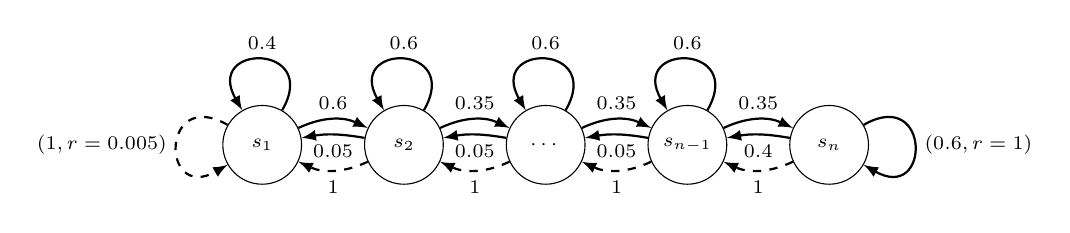
\begin{tikzpicture}[
  >=latex,
  x=12mm, y=10mm,           % Slightly reduced spacing for single-column fit
  state/.style={circle,draw,minimum width=10mm,inner sep=0.8pt, font=\scriptsize},
  Redge/.style={->,thick},  % Right action (solid)
  Ledge/.style={->,thick,dashed},
  every node/.style={font=\scriptsize} % Standardized font size for NeurIPS
]

% --- states (compacted for 5.5-inch column)
\node[state] (s1)   at (0,0) {$s_1$};
\node[state] (s2)   at (1.5,0) {$s_2$};
\node[state] (dots) at (3,0) {$\cdots$};   
\node[state] (snm) at (4.5,0) {$s_{n-1}$};
\node[state] (sn)   at (6,0) {$s_n$};

% ===== Solid edges: action R =====
% s1: self 0.4, to s2 0.6
\draw[Redge] (s1) edge[out=60,in=120,looseness=5] node[above] {$0.4$} (s1);
\draw[Redge] (s1) to[bend left=25] node[above,sloped] {$0.6$} (s2);

% s2: self 0.6, to the right 0.35, to left 0.05
\draw[Redge] (s2) edge[out=60,in=120,looseness=5] node[above] {$0.6$} (s2);
\draw[Redge] (s2) to[bend left=25] node[above,sloped] {$0.35$} (dots);
\draw[Redge] (s2) to[bend right=10] node[below,sloped] {$0.05$} (s1);

% dots: self 0.6, to the right 0.35, to left 0.05
\draw[Redge] (dots) to[bend left=25] node[above,sloped] {$0.35$} (snm);
\draw[Redge] (dots) edge[out=60,in=120,looseness=5] node[above] {$0.6$} (dots);
\draw[Redge] (dots) to[bend right=10] node[below,sloped] {$0.05$} (s2);

\draw[Redge] (snm) edge[out=60,in=120,looseness=5] node[above] {$0.6$} (snm);
\draw[Redge] (snm) to[bend left=25] node[above,sloped] {$0.35$} (sn);
\draw[Redge] (snm) to[bend right=10] node[below,sloped] {$0.05$} (dots);

\draw[Redge] (sn) to[bend right=10] node[below,sloped] {$0.4$} (snm);
\draw[Redge] (sn) edge[out=30,in=-30,looseness=5] node[right] {$(0.6,r=1)$} (sn);

% ===== Dashed edges: action L (probability 1) =====
\draw[Ledge] (s2)   to[bend left=25] node[below,sloped] {$1$} (s1);
\draw[Ledge] (dots) to[bend left=25] node[below,sloped] {$1$} (s2);
\draw[Ledge] (snm) to[bend left=25] node[below,sloped] {$1$} (dots);
\draw[Ledge] (sn)   to[bend left=25] node[below,sloped] {$1$} (snm);
\draw[Ledge] (s1) edge[out=150,in=210,looseness=5] node[left] {$(1, r=0.005)$} (s1);

\end{tikzpicture}

\end{document}